\documentclass{article}

\usepackage{graphicx, xcolor}
\usepackage{amsmath, amssymb}
\usepackage[colorlinks=true,allcolors=blue]{hyperref}

\usepackage[margin=1in]{geometry}

\def\hwtitle{Homework 3: Ordinary Differential Equations, Part 1}
\def\hwauthor{Caden Gobat}
\def\hwdate{\today}

\usepackage{fancyhdr}
\lhead{\hwauthor}
\chead{\hwtitle}
\rhead{\hwdate}
\lfoot{\hwauthor}
\cfoot{}
\rfoot{\thepage}
\renewcommand{\footrulewidth}{0.4pt}
\pagestyle{fancy}

\author{\hwauthor}
\title{\hwtitle}
\date{\hwdate}

\begin{document}

\maketitle
\thispagestyle{fancy}

\section{Introduction}

Last week we explored some simple integration techniques for evaluating ODEs numerically. This week we will use a second-order Runge-Kutta method to solve the differential equation of motion due to gravity. Newton tells us that the magnitude of the gravitational force between the Sun and Earth is $\displaystyle F_G=\frac{GM_\odot M_\oplus}{R^2}$. We also know from his second law that the Earth will move around the Sun with an accerlation described by $\vec{F}=M_\oplus \mathbf{a} = M_\oplus \ddot{\mathbf{x}}$. Thus, solving for the acceleration gives $\displaystyle \ddot{\mathbf{x}} = \frac{GM_\odot}{R^2}$, which can also be written as \begin{equation} \label{eq:gravity}
    \ddot{\mathbf{r}} = \frac{GM_\odot}{r^2}(-\hat{\mathbf{r}})    
\end{equation}
where $\mathbf{r}=\langle x,y\rangle$ and $r = \sqrt{x^2+y^2}$.

The second-order Runge-Kutta formula (RK2) is as follows: \begin{align*}
    \frac{d\phi}{dt} &= f(\phi,t) \\
    k_1 &= \Delta t \cdot f(\phi_n,t_n) \\
    k_2 &= \Delta t \cdot f\left(\phi_n+\frac{k_1}{2}, t_n+\frac{\Delta t}{2}\right) \\
    \phi_{n+1} &= \phi_n + k_2
\end{align*}
where in this case $\phi$ is a 4-element vector made up of $\langle x,y,v_x,v_y\rangle$ and $f$ is the derivatives function that uses Eq.~\ref{eq:gravity} to calculate velocity based on acceleration and position based on velocity (\emph{this} equation is time-independent, but it is possible that the derivatives function could depend on the actual time $t$ as well). In this report I showcase some of the results that an implementation of this algorithm in \texttt{C} is capable of producing.

\section{Results}

\bigskip
\noindent{\bf Question 1}
\medskip

\begin{itemize}
    \item $GM_\odot$ in ``Earth orbit'' units (AU and years) has a numerical value of $(2\pi)^2=4\pi^2\approx39.4784$
    \item Assuming an ideally circular orbit, Earth must travel a distance of $2\pi(1 \text{ AU})$ in a year. Thus its tangential velocity is simply $2\pi\ \frac{\text{AU}}{\text{year}}$.
\end{itemize}

\newpage
\bigskip
\noindent{\bf Question 2}
\medskip

\begin{figure}[h!]
    \centering
    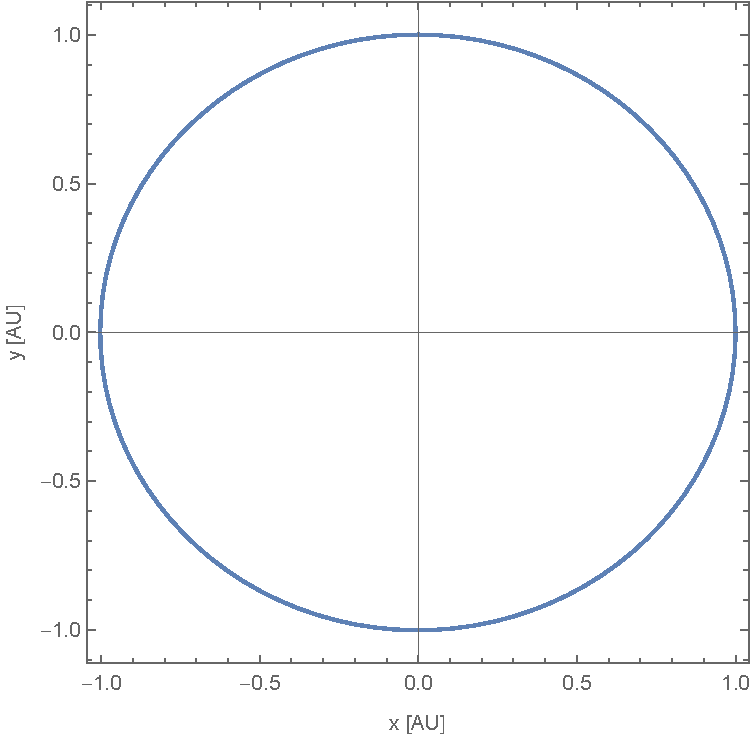
\includegraphics[width=3.5in]{homework3/q2_orbit.pdf}
    \caption{Using the initial conditions discussed in \textbf{Question 1}, we can simulate an orbit for the Earth that is approximately circular over the course of a year, as anticipated.}
    \label{fig:q2orbit}
\end{figure}

\begin{figure}[h!]
    \centering
    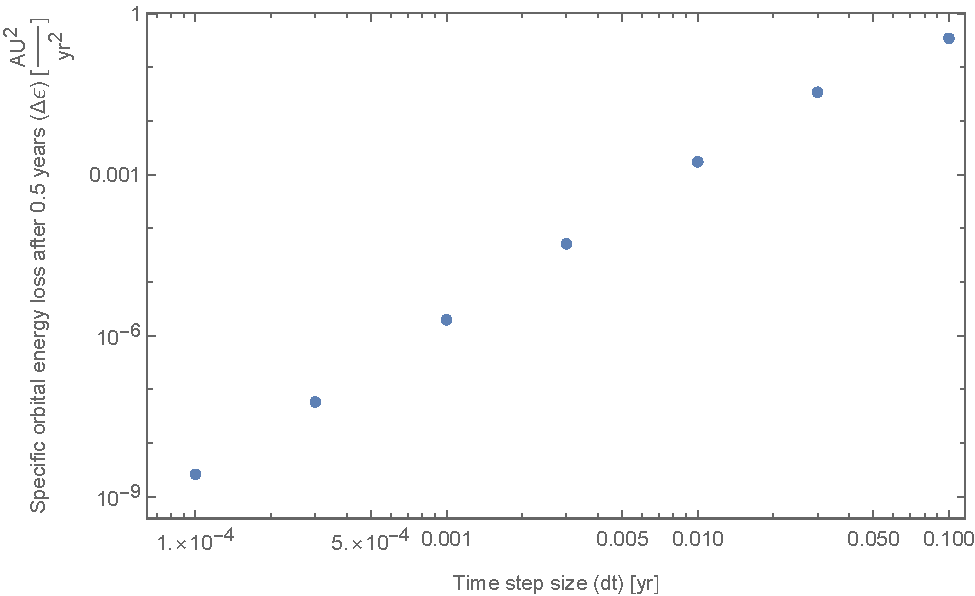
\includegraphics[width=5in]{homework3/q2_energyloss.pdf}
    \caption{Specific orbital energy per unit mass lost after half a year of simulation using various step sizes ($dt$). Larger steps lead to greater non-conservation of energy. Log slope is approximately 2.781, meaning this algorithm converges even faster than $\mathcal{O}(n^2)$ (since $n\propto1/dt$), which is what is expected.}
    \label{fig:q2energy}
\end{figure}

In order to attain an error of $\lesssim0.001$, we need a $dt$ of just under 0.01 years.

\newpage
\bigskip
\noindent{\bf Question 3}
\medskip

\begin{figure}[h!]
    \centering
    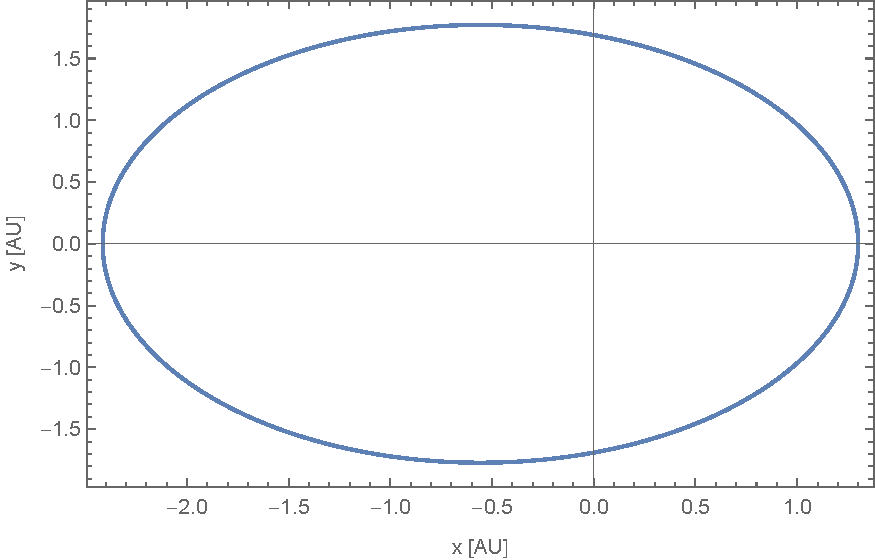
\includegraphics[width=5in]{homework3/q3_orbit.pdf}
    \caption{Trajectory of an eccentric orbit using $(x_0,y_0)=(1.3,0)$; $(v_{x,0},v_{y,0}=(0,2\pi)$; and $dt=0.001$ yr.}
    \label{fig:q3orbit}
\end{figure}

This orbiting body starts at perihelion, or $R_\text{min}$, of 1.3 AU. It reaches a maximum distance (aphelion) of 2.414 AU, meaning the ratio is $\frac{r_a}{r_p}=1.857$.

\begin{figure}[h!]
    \centering
    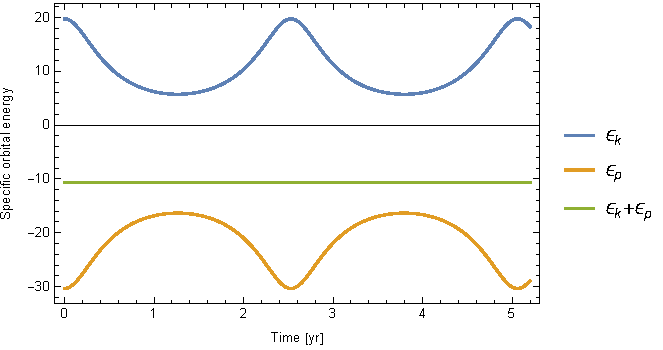
\includegraphics[width=5in]{homework3/q3energy.pdf}
    \caption{Orbital energies per unit mass, plotted over two complete periods. As expected, the total energy remains nearly constant, with potential and kinetic being converted back and forth into one another throughout the orbit. Furthermore, it also makes sense that kinetic energy is at a maximum at the closest approach to the Sun (when velocity is greatest), and potential is greatest when it is furthest away.}
    \label{fig:q3energy}
\end{figure}

\newpage
\bigskip
\noindent{\bf Question 4}
\medskip

\begin{figure}[h!]
    \centering
    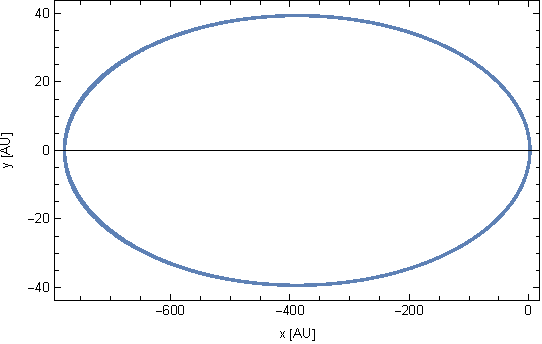
\includegraphics[width=5in]{homework3/q4orbit.pdf}
    \caption{Simulated trajectory of one complete orbit of a comet with $(x_0,y_0)=(1.995,0)$ and $v_0=2\pi$ AU/yr.}
    \label{fig:q4orbit}
\end{figure}

\begin{figure}[h!]
    \centering
    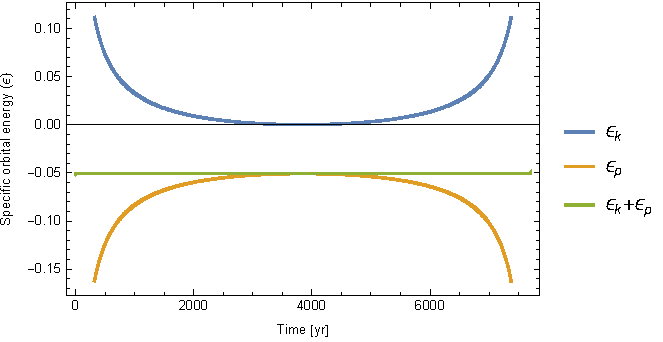
\includegraphics[width=5in]{homework3/q4energy.pdf}
    \caption{Orbital energy per unit mass for the comet whose trajectory is shown in Fig.~\ref{fig:q4orbit}. The timescale of the period is more apparent here, and the behavior whereby the total $\epsilon$ remains constant over time holds true.}
    \label{fig:q4energy}
\end{figure}

This setup yields a period of approximately $\boxed{7694\text{ years}}$ for this first revolution.

\newpage
\bigskip
\noindent{\bf Question 5}
\medskip

\begin{figure}[h!]
    \centering
    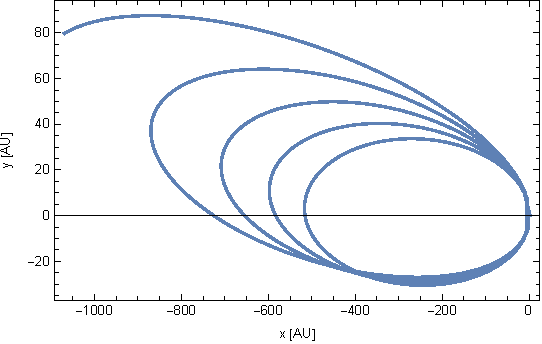
\includegraphics[width=5in]{homework3/q5orbit.pdf}
    \caption{Multiple orbits over a time domain of 30,000 years using the same initial conditions as in \textbf{Question 4}. Clearly, there is some error introduced over the course of several revolutions, as the simulation does not retrace the same path every time.}
    \label{fig:q5orbit}
\end{figure}

\begin{figure}[h!]
    \centering
    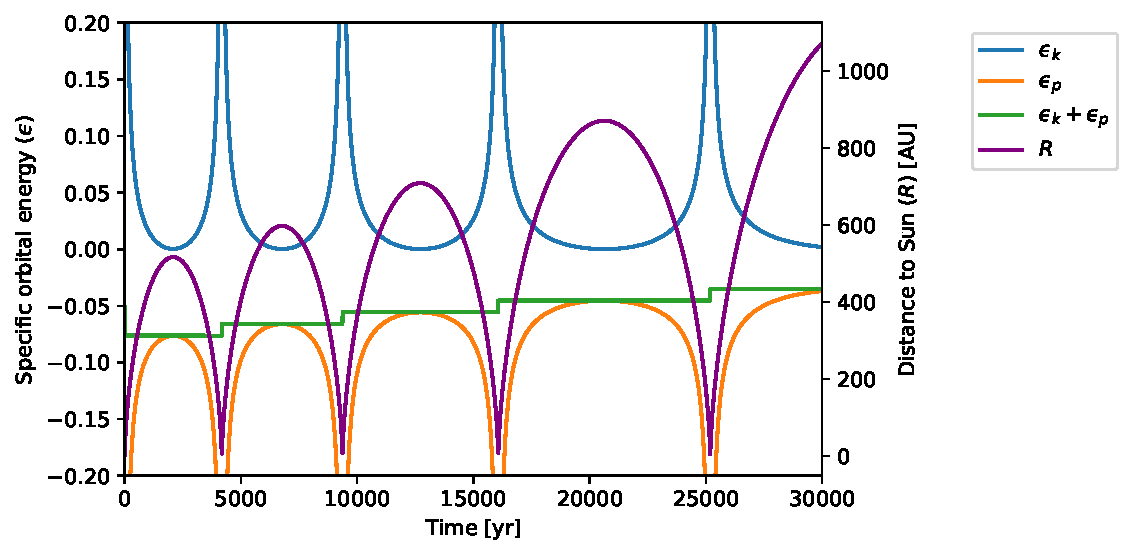
\includegraphics[width=5.5in]{homework3/q5energy.pdf}
    \caption{Specific orbital energy as plotted previously, but this time overlaid with distance from the Sun as a function of time as well. Here the total $\epsilon$ does not remain constant, as there is a bump up each time the comet reaches perihelion (the minimum distance to the Sun). This is because of the fact that in an orbit this eccentric, the velocity at perihelion is relatively much greater, so the step size (however small) is less capable of capturing all of the motion during the close approach as during the rest of the orbit, so the high velocity ``overshoots.'' This issue with the velocity causes an erroneous increase in kinetic energy at perihelion, which in turn increases the total energy and results in an increase in the size of the orbit with each consecutive period.}
    \label{fig:q5energy}
\end{figure}

\newpage
\section{Conclusions}

This assignment was a great introduction to higher-order numerical integration techniques, and involved a physically intriguing problem at the same time. I have done Runge-Kutta integration in Python in the past to simulate orbits, so implementing similar things in \texttt{C} was a fun exercise.

I did not have many significant challenges other than an initial misunderstanding of what \textbf{Question 2} was asking in regards to the non-conservation of $\epsilon$, but I was able to figure it all out.

I look forward to continuing to explore numerical methods.

\end{document}
